\documentclass{beamer}

\usepackage{ucs}
\usepackage[utf8x]{inputenc}
\usepackage[T1]{fontenc}
\usepackage[english]{babel}
\usepackage{epstopdf}

%\usepackage{multirow}%	multirow
%\usepackage[retainorgcmds]{IEEEtrantools}%	IEEEeqnarray
%\usepackage{mathabx}%	convolution symbol
\usepackage{relsize}%	relative font sizes
%\usepackage{listings}
%\usepackage{graphicx}
\usepackage{multicol}


%	presentation info
\title[OpenMP: analyze \& improve]{A finite volume case study from an industrial application}
\subtitle{OpenMP: analysis and improvements}

\author{M. Palhas \and P. Costa}

\institute[19808 \and 19830]{
	University of Minho\\
	Department of Informatics
}

\date{Braga, April 2012}


%	beamer options
\usetheme{CambridgeUS}


\begin{document}%	begin presentation

\maketitle%	title slide

\begin{frame}
	\frametitle{Index}
	\tableofcontents
\end{frame}

%\begin{frame}
%	\frametitle{Parallelization}
%	\begin{figure}
%		\begin{center}
%			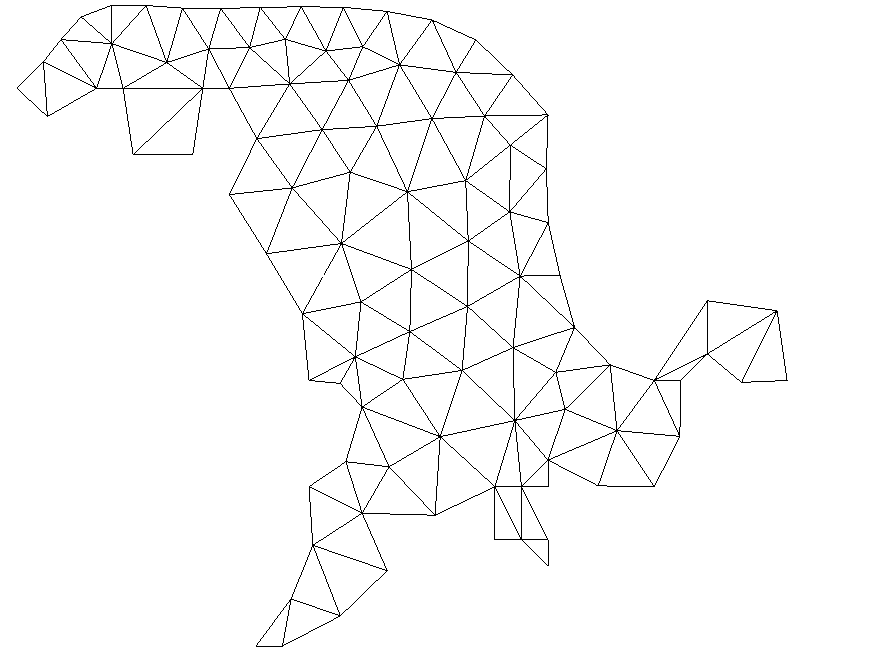
\includegraphics[height=0.8\textheight]{images/slides.march/mesh0.png}
%		\end{center}
%	\end{figure}
%\end{frame}
%
%\begin{frame}
%	\frametitle{Algorithm}
%	\begin{itemize}
%		\item{Heartbeat algorithm:
%		\begin{enumerate}
%			\item{Compute the pollution fluxes;}
%			\item{Update the pollution levels;}
%		\end{enumerate}
%		}
%		\item{\texttt{compute\_flux}
%		\begin{itemize}
%			\item{Iterate over \textbf{edges};}
%			\item{Dependency when calculating $\delta t$
%			\begin{itemize}
%				\item{Removed replacing with a sum reduction;}
%				\item{Implementation simplifications allow to remove this completely;}
%			\end{itemize}
%			}
%		\end{itemize}
%		}
%		\item{\texttt{update}
%		\begin{itemize}
%			\item{Originally iterate over \textbf{edges};}
%			\item{Race condition in \textbf{cells};
%			\begin{itemize}
%				\item{Removed changing to cell iterations;}
%				\item{Hurts locality;}
%			\end{itemize}
%			}
%		\end{itemize}
%		}
%	\end{itemize}
%\end{frame}

\section{Memory requirements}
\subsection{Computational intensity}
\begin{frame}
	\frametitle{Roofline}
	\begin{multicols}{2}
		\begin{figure}
			\begin{center}
				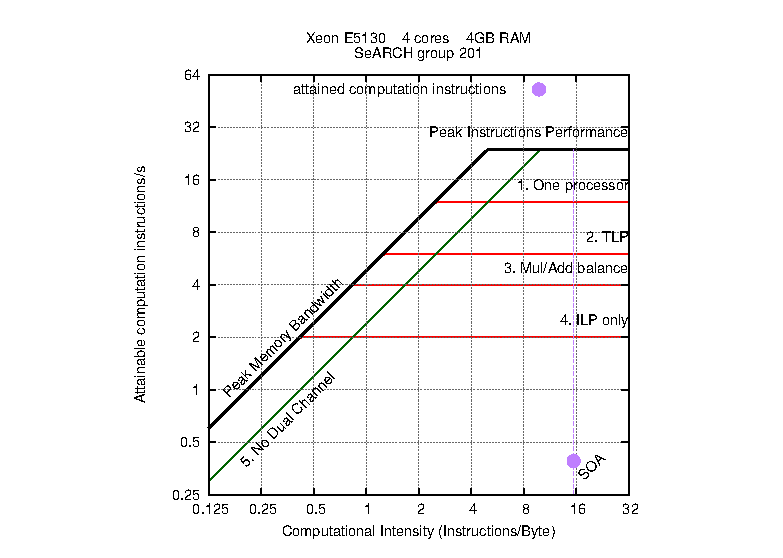
\includegraphics[width=0.75\textwidth]{images/roofline/201.eps}
			\end{center}
		\end{figure}
		\begin{description}
			\item[AOS]{8.20 Insts/Byte\\0.34 GInsts/s}
			\item[SOA]{15.49 Insts/Byte\\0.39 GInsts/s}
		\end{description}
	\end{multicols}
\end{frame}

\begin{frame}
	\frametitle{Comparing}
	\begin{center}
		\parbox{0.7\textwidth}{
			\begin{itemize}
				\item[]{Greater computational intensity;}
				\item[]{Equal amount of instructions per second;}
			\end{itemize}
		}
	\end{center}
	\begin{center}
		\Huge\bfseries
		Why?
	\end{center}
	\begin{itemize}
		\pause
		\item{Less bytes accessed?}
		\pause
		\item{More instructions?}
		\pause
		\item{Less time?}
	\end{itemize}
\end{frame}

\begin{frame}
	\frametitle{Less bytes accessed?}
	\begin{multicols}{2}
		\begin{figure}
			\begin{center}
				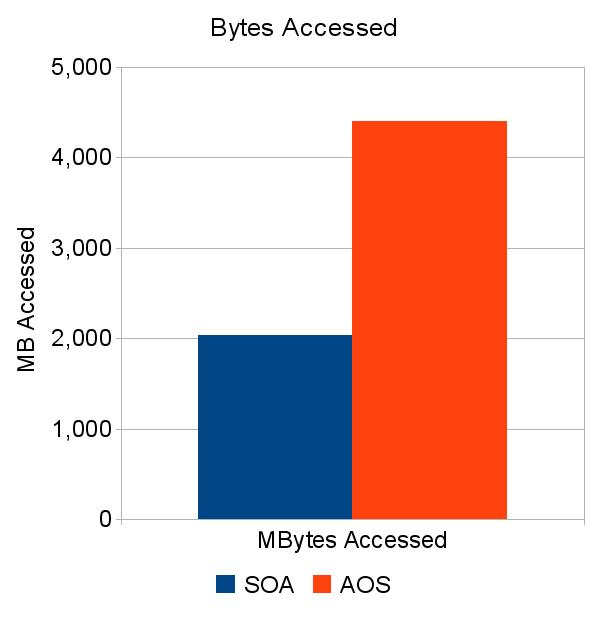
\includegraphics[width=0.5\textwidth]{images/slides.april/bytes.jpg}
			\end{center}
		\end{figure}
		
		\begin{center}
			\huge\bfseries YES
		\end{center}
		
		\textbf{Less than half} bytes accessed with SOA.
	\end{multicols}
\end{frame}

\begin{frame}
	\frametitle{More instructions?}
	\begin{multicols}{2}
		\begin{figure}
			\begin{center}
				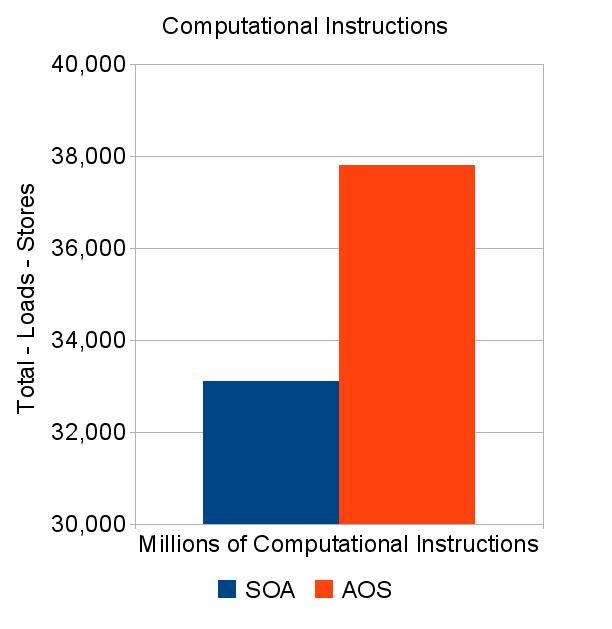
\includegraphics[width=0.5\textwidth]{images/slides.april/instructions.jpg}
			\end{center}
		\end{figure}
				
		\begin{center}
			\huge\bfseries NO
		\end{center}
		
		\textbf{7\% less} instructions in the SOA version.
	\end{multicols}
\end{frame}

\begin{frame}
	\frametitle{Less time?}
	\begin{multicols}{2}
		\begin{figure}
			\begin{center}
				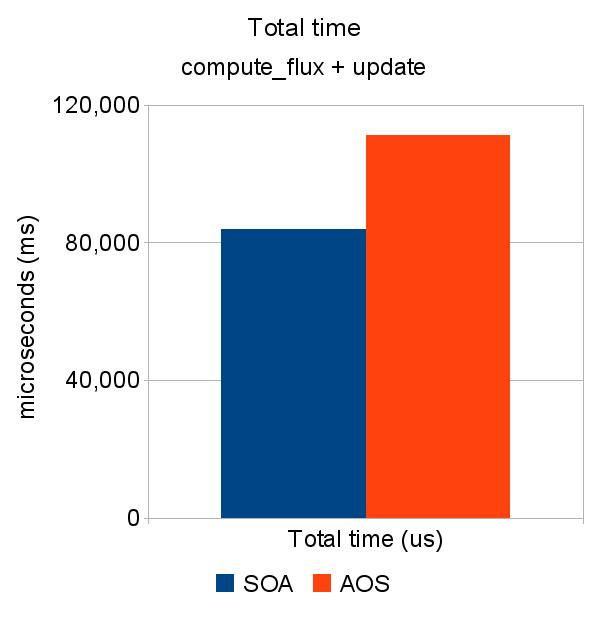
\includegraphics[width=0.5\textwidth]{images/slides.april/fnctime.jpg}
			\end{center}
		\end{figure}
				
		\begin{center}
			\huge\bfseries YES
		\end{center}
		
		\textbf{A speedup of 1.28} in the SOA version, when compared to the AOS version.
	\end{multicols}
\end{frame}

\subsection{Instruction Mix}
\frame{\tableofcontents[currentsection,currentsubsection]}
\begin{frame}
	\frametitle{AOS}
	\begin{figure}
		\begin{center}
			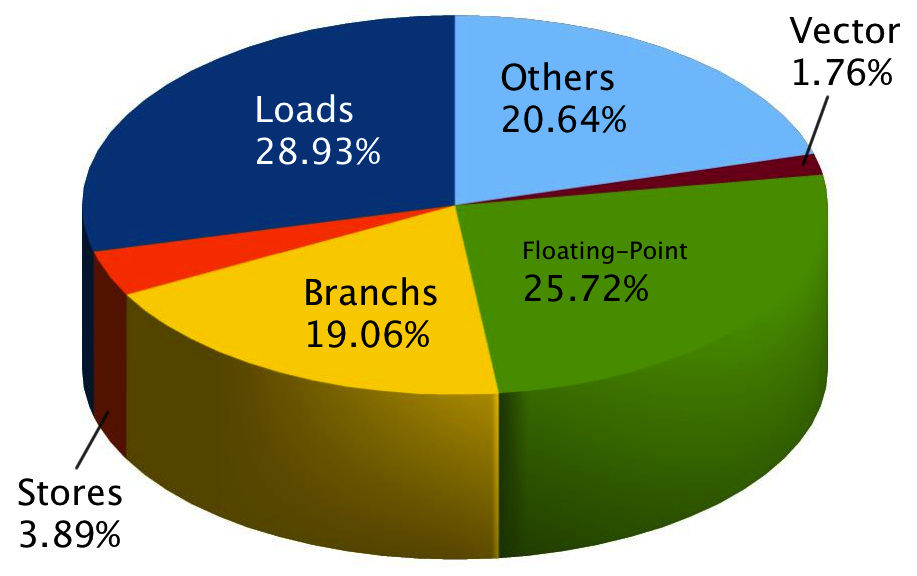
\includegraphics[width=0.9\textwidth]{images/slides.april/instmxAOS.png}
		\end{center}
	\end{figure}
\end{frame}

\begin{frame}
	\frametitle{SOA}
	\begin{figure}
		\begin{center}
			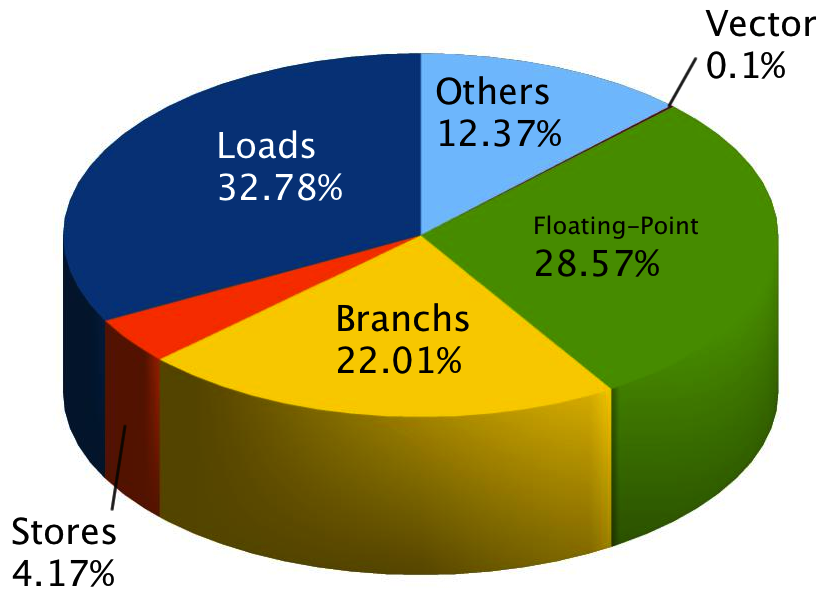
\includegraphics[width=0.85\textwidth]{images/slides.april/instmxSOA.png}
		\end{center}
	\end{figure}
\end{frame}

\begin{frame}
\frametitle{Instruction Mix}
	\begin{table}
		\begin{center}
			\begin{tabular}{|c|cc|}
				\hline
				\textbf{Instruction Type} & \textbf{AOS} & \textbf{SOA} \\
				\hline
				\hline
				Loads & 28.93\% & 32.78\% \\
				Stores & 3.89\% & 4.17\% \\
				Floating-Point & 25.72\% & 28.57\% \\
				Branchs & 19.06\% & 22.01\% \\
				Others & 20.64\% & 12.37\% \\
				\hline
			\end{tabular}
		\end{center}
	\end{table}
\end{frame}

\subsection{Cache}
\frame{\tableofcontents[currentsection,currentsubsection]}
\begin{frame}
	\frametitle{Miss Rates}
	\begin{figure}
		\begin{center}
			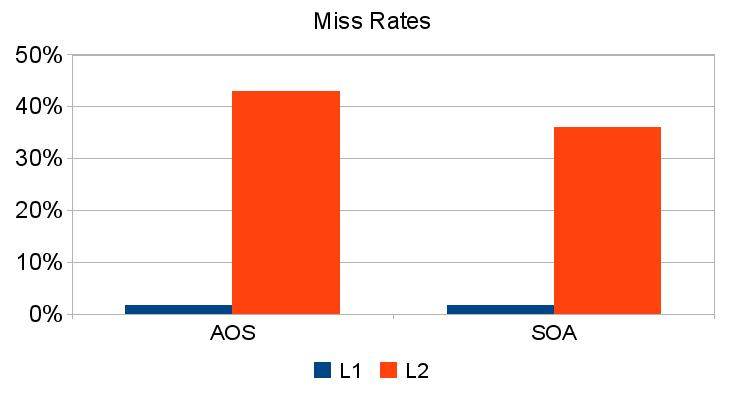
\includegraphics[width=0.7\textwidth]{images/slides.april/missrate.jpg}
		\end{center}
	\end{figure}
	\begin{itemize}
		\item{\textbf{1.71\%} miss rate in L1 for both versions;}
		\item{\textbf{Less 6.76\%} miss rate in L2 for the SOA version;}
	\end{itemize}
\end{frame}




\section{Granularity}
\frame{\tableofcontents[currentsection,currentsubsection]}
\begin{frame}
	\frametitle{Step Time}
	\begin{figure}
		\begin{center}
			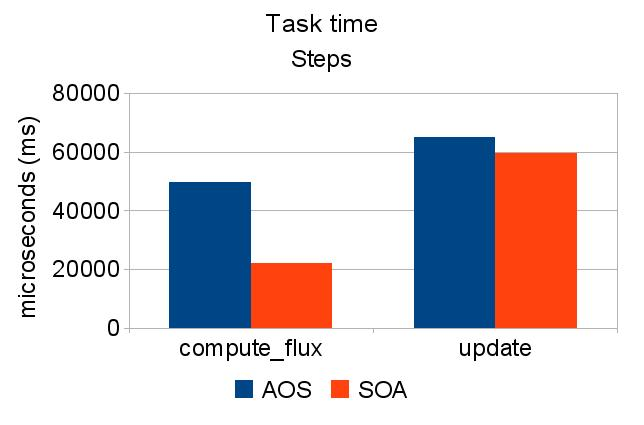
\includegraphics[width=0.6\textwidth]{images/slides.april/steps.jpg}
		\end{center}
	\end{figure}
	\begin{itemize}
		\item{OpenMP microbenchmarks:
		\begin{description}
			\item[\texttt{PARALLEL FOR}]{--- 2.85 $\mu$s overhead}
		\end{description}
		}
	\end{itemize}
\end{frame}


\section{Task balance}
\frame{\tableofcontents[currentsection,currentsubsection]}
\begin{frame}
	\frametitle{Action Time}
	\begin{figure}
		\begin{center}
			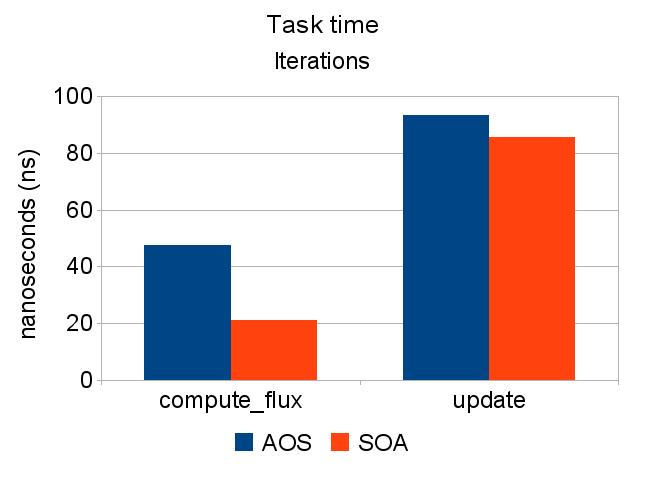
\includegraphics[width=0.6\textwidth]{images/slides.april/iterations.jpg}
		\end{center}
	\end{figure}
	\begin{itemize}
		\item{Each step has the same workload in each iteration.}
	\end{itemize}
\end{frame}


\section{Scalability}
\frame{\tableofcontents[currentsection,currentsubsection]}
\begin{frame}
	\frametitle{Speedups}
	\begin{figure}
		\begin{center}
			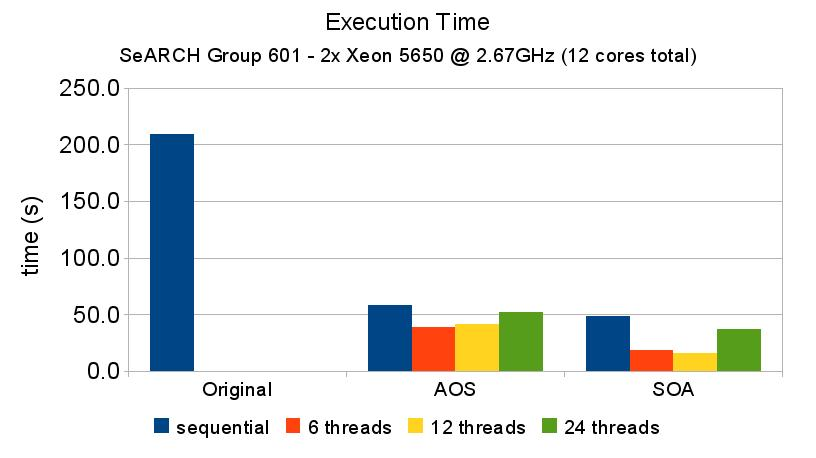
\includegraphics[width=0.85\textwidth]{images/slides.april/exectime.jpg}
		\end{center}
	\end{figure}
	\begin{description}
		\item[Best result:]{SOA version running in 12 cores (1 thread per core) --- \textbf{3.04 speedup}.}
	\end{description}
\end{frame}



\section{Conclusions}
\frame{\tableofcontents[currentsection,currentsubsection]}
\begin{frame}
	\frametitle{Conclusions}
	\begin{itemize}
		\item{Implementation remains memory bound;}
		\pause
		\item{\textit{Struct-of-Arrays} is a more efficient approach than \textit{Array-of-Structs};
		\begin{itemize}
			\item{Better, but locality problems remain;}
		\end{itemize}
		}
		\pause
		\item{Locality improvements may be achieved with a greater control over the mesh structure:
		\begin{itemize}
			\item{The \texttt{gmsh} program already generates a rather organized input;}
			\item{This organization is more suitable for a CUDA implementation;}
		\end{itemize}
		}
		\pause
		\item{Parallelizable tasks total time significantly greater than the OpenMP overhead;}
	\end{itemize}
\end{frame}
\begin{frame}
	\frametitle{Conclusions}
	\begin{itemize}
		\item{Synchronization only between the heartbeat phases;}
		\pause
		\item{The program is \textbf{heterogeneous};
		\begin{itemize}
			\item{\texttt{update} > \texttt{compute\_flux}}
		\end{itemize}
		}
		\pause
		\item{Each task is \textbf{homogeneous};}
		\pause
		\item{\texttt{gcc} seems to generate better code:
		\begin{itemize}
			\item{\texttt{gcc 4.1} generated faster code than \texttt{icc 11}, except when dealing with HyperThreading;}
			\item{The current version of \texttt{gcc} is \texttt{4.6} (some systems already have \texttt{4.7});}
			\item{Technical problems prevented further testing.}
		\end{itemize}
		}
	\end{itemize}
\end{frame}

\section{Questions}
\begin{frame}
	\titlepage
	\begin{center}
		\Huge\bfseries
		- ? -
	\end{center}
\end{frame}

\end{document}%	end presentation
